\subsection{Brugsmønsteranalyse}
Der vil i dette afsnit blive lavet en brugsmønsteranalyse på de detaljerede brugsmønstre fra afsnit \ref{section: detailed_usemodels}, der har til formål at finde klasse, finde struktur og finde adfærd i et system. Det første der gøres er at finde klasser:

\subsubsection{Klassekandidater}
Når man skal finde potentielle klasser, kan der tages brug af en navneordsanalyse, hvor man finder potentielle klasserkandidater. Nedenfor kan listen af potentielle klasser fra navneordsanalysen af brugsmønstrene ses i tabel \ref{table:class_candidates}.

\begin{table}[ht]
    \begin{tabularx}{\textwidth}{|p{4cm}|p{4cm}|X|}
        \hline
        \textbf{Klassekandidat} & \textbf{Attributter} & \textbf{Kommentar} \\
        \hline
        % Læs kreditering -----------------------------------------------------------
        \multirow{2}{*}{Bruger}      & \texttt{uuid}, \texttt{e-mail}, \texttt{password}, \texttt{rolle} & Indebærer alle aktørerne (Systemadmin, kanaladmin, producer og royalty bruger).\\
        \hline
        \multirow{2}{*}{Produktion}  & \texttt{uuid}, \texttt{titel}, \texttt{kanal\_id} & Et program indebærer alt hvad der bliver vist på TV. (Film, serier osv) \\
        \hline
        \multirow{3}{*}{Kreditering} & \texttt{person\_id}, \texttt{job}, \texttt{produktion\_id} & En kreditering er et job udført af en person til en produktion (hvor job  kan være lydmand) \\
        \hline
        % Opret Kreditering ---------------------------------------------------------
        \multirow{2}{*}{Kanal} & \multirow{2}{*}{\texttt{ID}, \texttt{navn}} & Angiver hvilken TV-kanal et program bliver afspillet på \\
        \hline
        % Opret Person --------------------------------------------------------------
        \multirow{3}{*}{Person} & Personinformation (navn, beskæftigelse, e-mail, tlf.nr. osv)  & De der medvirker til produceringen af en produktion (kameramand, lydmand, etc.)\\
        \hline
        % Log ud --------------------------------------------------------------------
            % Nur duplications
        %Log in ---------------------------------------------------------------------
            % Nur Duplications
        % Opret Producer ------------------------------------------------------------
            % Nur Duplications
        % Se personinformation ------------------------------------------------------
            % Nur Duplications
        % Godkend nye krediteringer -------------------------------------------------
    \end{tabularx}
    \caption{Klasssekandidater}
    \label{table:class_candidates}
\end{table}

% vi behøver ikke at bruge  mere :)

Her er der tildelt nogle attributter, blandt andet fra kasserede klassekandidater, som klasserne bør indeholde.

\subsubsection{Kasserede klassekandidater}
De resterende potentielle klasser der blev fundet under navneordsanalysen er enten synonymer, operationer eller egner sig bedre som attributter til de valgte potentielle klasser. Disse kan ses i tabel \ref{table:deleted_class_candidates}

\begin{table}[H]
    \begin{tabularx}{\textwidth}{|X|X|}
        \hline
        \textbf{Kasserede klassekandidater} & \textbf{Kommentar} \\
        \hline
        Gæst & Påvirker ikke systemet - Kan kun se krediteringerne\\
        \hline
        Systemet & Systemet  \\
        \hline
        Rolle   & Attribut til Bruger-klassen\\
        \hline
        Visning  & En Operation\\
        \hline
        Film & Synonym til Produktion-klassen\\ 
        \hline
        Program & Synonym til Produktion-klassen\\ 
        \hline
        Knap & En del af Desktop-klienten\\
        \hline
        Programtitel & Attribut til Program-klassen\\
        \hline
        Vedkommende & Synonym for Bruger-klassen\\
        \hline
        Aktøren &  Synonym for Bruger-klassen\\
        \hline
        Person-vinduet & En del af Desktop-klienten\\
        \hline
        Informationer (navn, beskæftigelse, email, tlf.nr., osv.) &  Attributter til Person-klassen\\
        \hline
        Oprettelse & En operation \\
        \hline
        Desktopklienten &  Systemet\\
        \hline
        Startsiden &  En del af Desktop-klienten\\
        \hline
        Login-side & En del af Desktop-klienten\\
        \hline
        Login-oplysninger & Attribut til Bruger-klassen\\
        \hline
        Brugernavn & Attribut til Bruger-klassen\\
        \hline
        Password & Attribut til Bruger-klassen\\
        \hline
        Flow & Beskriver et hændelsesforløb\\
        \hline
        Navn & Attribut \\
        \hline
        Primær aktør &  Synonym for Bruger-klassen\\
        \hline
        Personinformation &  Attributter til Person-klassen\\
        \hline
        Godkendelse & En operation \\
        \hline
        Meddelelse & En operation \\
        \hline
        Systemadministrator & En rolle i systemet - bliver håndteret af Bruger-klassen \\
        \hline
        Kanaladministrator & En rolle i systemet - bliver håndteret af Bruger-klassen \\
        \hline 
        Producer & En rolle i systemet - bliver håndteret af Bruger-klassen \\
        \hline
        Royalty Bruger & En rolle i systemet - bliver håndteret af Bruger-klassen \\
        \hline
    \end{tabularx}
    \caption{Kasserede klassekandidater}
    \label{table:deleted_class_candidates}
\end{table}


Her er det besluttet, at kandidaterne 'Brugernavn' og 'Password' begge er attributter til brugerklassen, og kandidaten 'Gæst' ikke skal være en klasse for sig, da denne klassekandidat kun kan se krediteringerne. Gæster skal ikke have specielle rettigheder eller login-oplysninger, som brugernavn og password.


\subsubsection{Klassekategori koncept}
De potentielle klasser der arbejdes videre med kan opdeles i kategorier. Dette er med til at skabe et overblik over klassernes ‘placering’ i systemet samt skabe associationer mellem koncepter og potentielle klasser.
Kategorilisten kan ses i tabel \ref{table:class_categories}.

\begin{table}[H]
    \begin{tabularx}{\textwidth}{|X|X|}
        \hline
        \textbf{Klassekategori koncept} & \textbf{Eksempel} \\
        \hline
        Forretnings overførsel & Ingen\\
        \hline
        Overførselslinje ting & Ingen\\
        \hline
        Produkt & Ingen \\
        \hline
        Hvor bliver overførslen optaget  & Ingen \\
        \hline
        Folkets roller & System- \& kanaladministrator, Producer, Royalty Bruger\\
        \hline
        Sted for overførsel & Ingen \\
        \hline
        Bemærkelsesværdige begivenheder & Ingen \\
        \hline
        Fysiske objekter & Ingen \\
        \hline
        Beskrivelse af ting & Krediteringer\\
        \hline
        Kataloger & Database med krediteringer\\
        \hline
        Lager af ting & Databasen\\
        \hline
        Ting på lageret & Krediteringer\\
        \hline
        Andre samarbejdssystemer & Ingen\\
        \hline
        Optagelser af finans, arbejde, kontrakter og juridiske sager & Ingen \\
        \hline
        Finansielle instrumenter & Ingen\\
        \hline
        Arbejdsplaner, manualer, dokumenter der er regulært refereret til for at performere arbejde & Ingen\\
        \hline
    \end{tabularx}
    \caption{Klassekategorier}
    \label{table:class_categories}
\end{table}

\subsubsection{Beskrivelse af klasser}
I tabel \ref{tab:user_class_description} er der givet et eksempel på, hvordan hver klasse kan komme til at se ud. De resterende kan findes i bilagene.
 
% ------------------------- Bruger --------------------------------
\begin{table}[H]
    \begin{tabularx}{\textwidth}{|p{3cm}|X|}
        \hline
        \textbf{Navn} & Bruger\\
        \hline
        \textbf{Definition} &  En bruger har et UUID, en email-adresse, et password og en rolle. \\
        \hline
        \textbf{Eksempel} & En bruger kan se ud som følgende: \\
                          & \texttt{UUID}: fbf50f43-9f1c-41e1-abce-cca32b836ef0 \\
                          & \texttt{Email}: someperson@somemail.com\\
                          & \texttt{Password}: Passw0rd\\
                          & \texttt{Rolle}: Kanaladministrator \\
        \hline
        \textbf{Andet} & Nej\\
        \hline
    \end{tabularx}
    \caption{Beskrivelse af Bruger-klassen}
    \label{tab:user_class_description}
\end{table}

\subsubsection{Analysemodel}


Ud fra navneordsanalysen er de potentielle klasser og deres attributter fundet. Dette vises i analysemodellen, som kan ses på figur \ref{fig:analysemodel} , med tilhørende relationer mellem klasserne. Modellen har til formål at danne et overblik over klasserne, deres attributter og deres relationer i systemet, samt at fungere som en model der kan bruges til videreudvikling af systemet. \\

\begin{figure}[h]
\centering
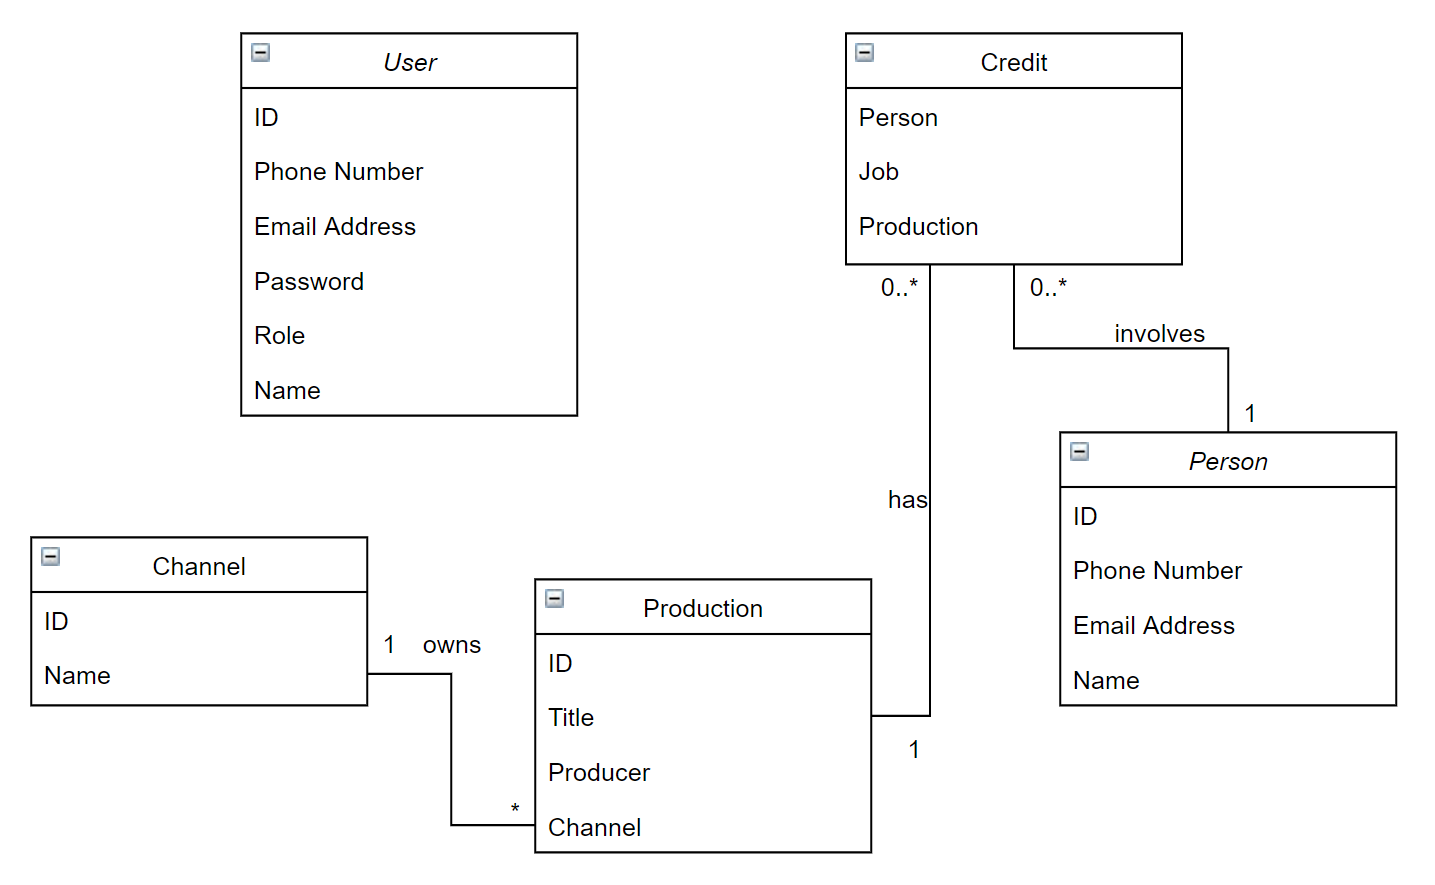
\includegraphics[scale=0.45]{figures/analysemodel.png}
\caption{Analysemodel}
\label{fig:analysemodel}
\end{figure}